\documentclass{article}

% ready for submission
\usepackage[preprint, nonatbib]{neurips_2022}

\usepackage[utf8]{inputenc} % allow utf-8 input
\usepackage[T1]{fontenc}    % use 8-bit T1 fonts
\usepackage{hyperref}       % hyperlinks
\usepackage{url}            % simple URL typesetting
\usepackage{booktabs}       % professional-quality tables
\usepackage{amsfonts}       % blackboard math symbols
\usepackage{nicefrac}       % compact symbols for 1/2, etc.
\usepackage{microtype}      % microtypography
\usepackage{xcolor}         % colors

\usepackage{amsmath, amssymb, amscd, amsthm, amsfonts}
\usepackage{mathtools}
\usepackage{enumerate}
\usepackage{float}
\usepackage{caption}
\usepackage{subcaption}
\usepackage{pythonhighlight}

\title{3D-SARI: 3D Stylized Avatars from a Rendered Image}

\author{%
  Mahir Kothary\\
  Computer Science\\
  Cornell Tech\\
  NYC, NY 10044 \\
  \texttt{mk942@cornell.edu} 
 \And Anna Pfohl\\
  Computer Science\\
  Cornell Tech\\
  NYC, NY 10044 \\
  \texttt{als462@cornell.edu}
\AND
  Gustavo Vasquez \\
  Computer Science\\
  Cornell Tech\\
  NYC, NY 10044 \\
  \texttt{av384@cornell.edu}
\And
  Jia Zhao \\
  Computer Science\\
  Cornell Tech\\
  NYC, NY 10044 \\
  \texttt{jz538@cornell.edu}
}

\begin{document}

\maketitle


\begin{abstract}
In this paper we present 3D Stylized Avatars from a Rendered Image (3D-SARI), a mechanism to generate a stylized 3D avatar from a single clothing reference and a style reference image. Existing methods in fashion have used 3D models to create virtual try-on projections or have used style transfer to generate new 2D fashion items from a style reference image and a segmented outfit. Our novel method combines both Monocular-to-3D projections for virtual try-on projections and style transfer for fashion design to generate 3D clothed avatars.
\end{abstract}


\section*{Todo}
1. change project name \\ 
2. more shirts / style transfer samples - Jia - done\\ 
3. Run model again (make some look good) - Mahir  \\
4. Review methods \& model section - Mahir/Jia \\ 
5. Create survey + gifs - Anna \\
6. limitations (shirt size, clothing styles, skin tones, ) \& ethics and bias of the model - Gus \\ 
7. future work (more recent papers) - Anna \\


\section{Introduction}
% What is the problem you are working on and why is it important? 
Fashion design is the art of applying design, style and textiles to create clothing articles such as dresses, suits, shoes, and bags. The intensive requirements of training and creativity in fashion design limits the general community from designing their own clothing. The process of designing a 2D clothing and fitting it onto a 3D human model has been empowered by computer vision techniques such as style transfer and 3D modeling. Increasing attention has raised in this process for its commercial value in real world fashion design and its potential in virtual avatar design in gaming and the metaverse.

Several prior works have explored 2D fashion design using segmentation and different style transfer models and GANs. MMFashion\cite{liu2021fashionVisTool} and fashion segmentation\cite{wang2020fashionSegmentation} understand and visualize fashion items and further segment the fashion items from a person wearing them. More advanced technologies have built on these systems to use the segmentation to help generate clothing try-on mechanisms\cite{Pang2021tryon, Tiwari2021tryon}. Artwork generated using state-of-the-art image techniques are already impressive to human eyes, but fashion design using the same techniques poses an interesting challenge due to limits of fine-grained details in 2D images. Novel research leveraging 3D modeling has provided a new approach to recover and reconstruct fine-grained clothing details in 3D virtual try-on projections. The aim of this paper is to explore fashion design on 3D models using  paint 2D fashion clothing generated by style transfer onto 3D reconstructions of human models.  


\subsection{Related Work}
% What’s been done on the problem so far? What methods have been tried? Can you list papers that have done similar things and talk about that? 

\textbf{Style Transfer} Style transfer learns the style of one image (e.g. art piece by Jackson Pollock), and applies it to a target image while preserving the content of the target image. The problem of style transfer is closely related to texture synthesis and rendering, which requires an explicit separation of image content from style. Early approaches\cite{Hertzmann2001st, Ashikhmin2003st} often failed on the separation due to the lack of image representations for semantic information. Style transfer became achievable after Gatys et al. proposed the seminal algorithm mapping the semantic features to convolutional layers and demonstrated that image content and image style can be separated and recombined \cite{gatys2016styleTransfer}. 

\textbf{Style Transfer Using GANs} GANs consist of a discriminator and a generator that competitively process backpropagation signals to learn deep representations with only a relatively small amount of training data \cite{creswell2018GANoverview, goodfellow2014GAN}. The adversarial loss of the discriminator will force the generator to generate images indistinguishable from real images. This characteristic of GANs has advanced image generation \cite{denton2015deepGAN, radford2015unsupervisedGAN}. Fashion design seems like an unexplored world for style transfer. Current research mainly focuses on virtual try-on with white background and the generated clothes are usually in simple patterns \cite{liu2021fashionVisTool, kato2019ganClothing, yildirim2019customOutfits}. More interesting research such as \cite{wang2020fashionSegmentation} leverages image segmentation to identify the clothing in a more complicated background and transfers the style to artistic work with relatively high resolution. However, GANs are computation intensive and the results of GAN-based fashion design are not satisfying to human eyes due to the limits of fine-grained details in 2D images.

\textbf{3D Modeling} High-fidelity 3D reconstruction with fine details of humans is the key to 3D fashion design. Previous approaches usually require expensive professional camera systems to capture the objects from multi views. Facebook researchers proposed an alternative with an end-to-end trainable framework in PIFuHD \cite{saito2020PIFuHD} to reconstruct clothed humans at high resolution from a single image without post-processing. In a more recent work \cite{zhureef}, Zhu et al. proposed ReEF to reconstruct clothing with surface details such as drape and winkles from clothes humans in single images. With fine-grained surface details, model M3D-VTON \cite{m3dvton} converts 2D clothing images to 3D try-on with multi views. The transformer-inspired StyleFormer proposed in \cite{wu2021styleformer} is a visually real-time style transfer method and generates coherent textures with fine details. 


% \textbf{Transformers} Transformers were initially designed for NLP tasks, but has started to gain better accuracy in vision tasks including segmentation, image classification and visual reasoning compared to the state-of-the-art CNN architectures \cite{khan2021CVtransSurvey}. Novel research in past months has demonstrated that, overall, transformers perform much more efficiently than CNNs with the same data sets and finetuning procedures \cite{malpure2021finetuneTrans}. StyTr2 proposed by \cite{deng2021stytr} is the first transfermor-based style transfer with encoders for both image content and image style. Transformer-based texture synthesis in style transfer has shown better result in \cite{lu2022transTextureSynthesis} compared to CNN-based models. 


\section{Methods}
% What are you going to do? Are you going to compare methods? Are you going to change methods? What methods  will you be comparing to? What metrics will you use to know if you succeed?

% You should list the questions the project will address and that will be discussed in the report.

\begin{figure}[H]
    \centering
    % todo: update samples in diagram
    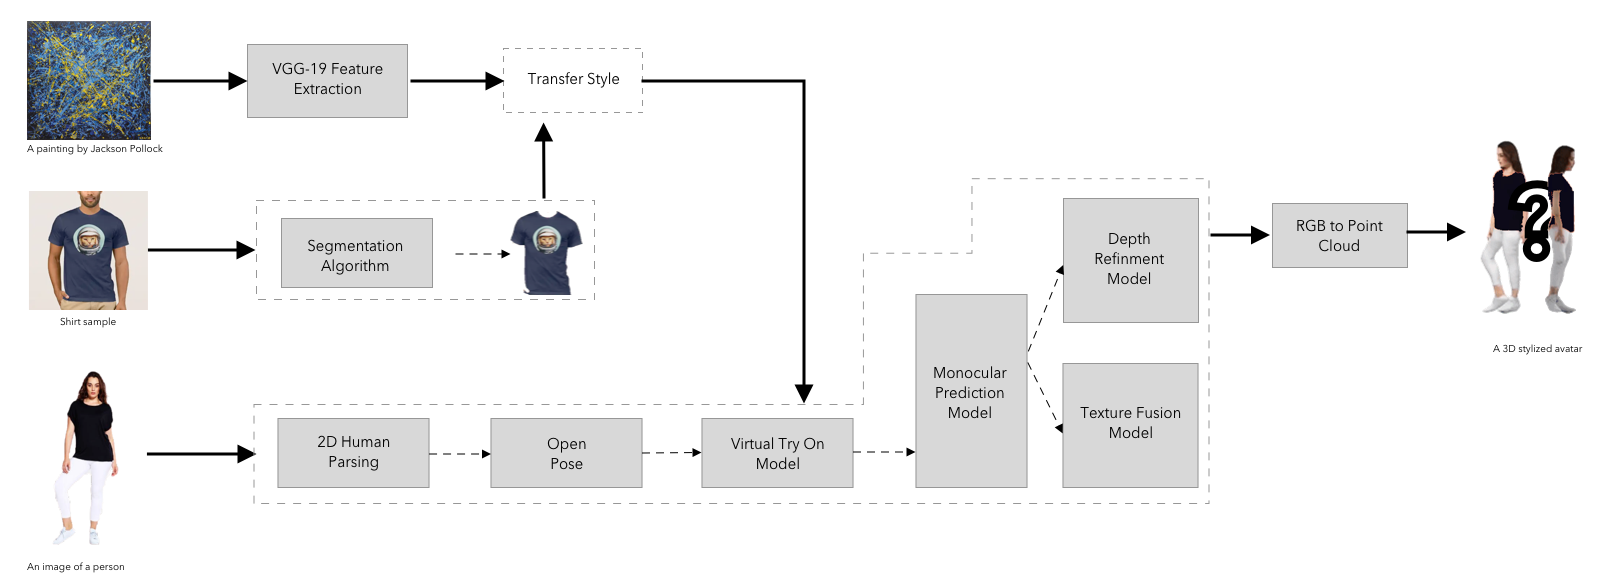
\includegraphics[width=\textwidth]{report/diagrams/3d_sari_2.png}
    \caption{System architecture: Our architecture is broken into four components, the style transfer, segmentation, pose keypoint detection and 3D rendering (which includes 3 submodules). Above, we use style transfer to extract features from the style to the reference fashion image. We provide an additional photo of a pose that is fed into segmentation of keypoint detection. All of these outputs are sent through the 3d rendering model to produce a three dimensional stylized point cloud}
\end{figure}

\subsection{Models}
\textbf{Style Transfer}
All content images and style images are resized to 512x512x3 to maintain size consistency in the model. Each content image has one clothing of white and background of black. The mask of each content image is created based on color values (black or white) to capture the contour of the clothing. This mask is used in the postprocessing step to get rid of style patterns beyond the contour of the clothing. 

Prior models from Gatys et al.\cite{gatys2016styleTransfer} have successfully used style transfer using art and applied them to other reference images. These have primarily been done using pre-trained VGG-models to extract key features from the style image, and applying it to the subject image. We aim to continue building on the same model, using the VGG-19 model to extract key features from our style images and applying them to generate stylized fashion pieces. 

\textbf{Segmentation}: We use the 2D Human Parsing library\cite{2dhumanparsing} which is a deep convolutional neural network known for performing well on image segmentation tasks\cite{2dsegmentation}.

\textbf{Pose Keypoint Detection}: We use the openpose\cite{openpose1}\cite{openpose2} library which uses Part Affinity Fields (PAFs) to identify body, hand, and face keypoints within the pose image.

\textbf{3D Rendering}: Zhao et al. released M3D-VTON\cite{m3dvton} with the purpose of providing a comprehensive three-pronged model to allow a 2D monocular image of a person to be converted into a 3D image, while taking into account the texture and fitting of the fashion piece. We use the pre-trained models for Monocular Prediction module (MPM), which is required to generate a clothes agnostic version of the person, and Depth Refinement module (DRM) to capture the angle and pose of the person. Lastly, we combine M3D-VTON's Texture Fusion module (TFM) with the style transfer model mentioned previously to generate clothing which is warped to fit the generated pose. Output depth values can then be rendered into a point cloud that represents the person and clothing in 3D space.

\subsection{Dataset}
% Describe the datasets you will use 
Because we will rely heavily on assembling pre-trained models, we will avoid needing to do large amounts of training. The models we will use will have already been trained on the MPV-3D dataset\cite{dong2019data1}. To collect samples for inference, we rely on the Kaggle \href{https://www.kaggle.com/datasets/ikarus777/best-artworks-of-all-time}{Best Artworks of All Time} datasets for art styles, and manually scrapped fashion articles from \href{https://www.farfetch.com}{www.farfetch.com} and model full body portraits from \href{https://www.modelscouts.com}{www.modelscouts.com}. Backgrounds were removed from the images using \href{https://www.remove.bg/}{www.remove.bg}

\subsection{Evaluation}
% Describe the hypotheses you will test and the related work. how will you know if the project is successful.
% To evaluate our model's success, we plan to use a combination of the Structural SIMilarity index measure (SSIM)\cite{wang2015eval}, the Frechet Inception Distance (FID)\cite{salimans2016eval}, and human evaluation (HE) similar to the M3D-VTON evaluation methods\cite{m3dvton}. As discussed by Gatys\cite{gatys2016styleTransfer} and others\cite{borji2018eval}\cite{zhou2019hype}, evaluating the success of style transfer models can be highly subjective so we plan to leverage HE for evaluation and comparison against the model benchmark listed above. We plan to send out randomized surveys to the Cornell Tech community that will assess the output of our model by ranking models against each other and output across different dimensions (e.g. realism, quality of texture, similarity to style reference etc). Our hypothesis is that are model combination methods will be more successful for stylized 3D renderings than the benchmarks alone, and results will be comparable to the 2D rendering models but in three dimensions.

\section{Results}

\section{Discussion}
% Ethics & bias

\section{Conclusion}

\subsection{Future work}

\section*{Contribution Statement}
All members contributed to coding and writing. Specifically:
\begin{enumerate}
\item Person: Did this and this
\end{enumerate}

\bibliographystyle{ieeetr}
\bibliography{ref}
\end{document}
